% Opciones empleadas:
%
%	a4paper -> indica el tamaño del papel, en este caso A4.
%	11pt -> tamaño de la fuente 11 puntos.
%	oneside -> sólo escribimos en una cara del folio.
% 
% Otras opciones interesantes:
%
%	twoside -> escribimos a doble cara.
%	openbib -> para que las referencias bibliográficas tengan un salto de línea entre cada campo de la referencia.
%
\documentclass[a4paper,11pt,twoside]{book}

% configuración de márgenes
\usepackage{setspace}
\doublespacing
\setlength\textwidth{15cm}
\setlength\textheight{22cm}
\setlength\oddsidemargin{1cm}
\setlength\evensidemargin{0cm}

% codificación utf8x y símbolos del idioma español (ñ, acentos, ...)
% el documento será necesario editarlo en utf-8
\usepackage[spanish]{babel}
\usepackage[utf8x]{inputenc}
\usepackage{morefloats}

% puede que queramos usar el símbolo del euro.
\usepackage{eurosym}

% El paquete fancybox nos permite crear cajas de diferentes estilos con facilidad.
% http://www.ctan.org/get/macros/latex/contrib/fancybox/fancybox.pdf
% http://www.mackichan.com/index.html?techtalk/487.htm~mainFrame
\usepackage{fancybox}
\usepackage{multicol}
\usepackage{amsmath}

% Para incluir subfiguras.
\usepackage{subfigure}

% Para incluir gráficos en JPG => compilar con pdflatex.
%\usepackage[pdftex]{graphicx}

% Para incluir gráficos EPS => compilar con latex.
\usepackage[dvips]{graphicx}

% Para escribir en color...
%
% ... cuando compilamos con el comando ``latex''
\usepackage[dvips,usenames]{color}
% ... uando compilamos con el comando ``pdflatex''
% \usepackage[pdftex,usenames,dvipsnames]{color}

% Para realiza hiperenlaces
\usepackage[pagebackref=true]{hyperref}
\hypersetup{
    bookmarks=true,         % barra de marcadores
    unicode=false,          % caracteres non-Latin en marcadores de Acrobat
    pdftoolbar=true,        % mostrar barra de herramientas de Acrobat
    pdfmenubar=true,        % mostrar menú de Acrobat
    pdffitwindow=false,     % ajustar ventana al ancho de página
    pdfstartview={FitH},    % ajustar documento al ancho de página
    pdftitle={Memoria PFG},    % título
    pdfauthor={},     % autor
    pdfsubject={},   % tema del documento
    pdfcreator={},   % generador del documento
    pdfproducer={}, % productor del documento
    pdfkeywords={}, % lista de palabras clave
    pdfnewwindow=true,      % enlaces en una nueva ventana
    colorlinks=true,       % false: enlaces en caja; true: enlaces coloreados
    linkcolor=blue,          % color de enlaces internos
    citecolor=green,        % color de enlaces a bibliografía
    filecolor=magenta,      % color de enlaces a ficheros
    urlcolor=blue           % color de enlaces externos
}

% Espaciado y ajuste de márgenes
\usepackage{setspace}
\onehalfspacing
% \doublespacing
\setlength{\textwidth}{15cm}
\setlength{\textheight}{22cm}

% Para evitar lineas huérfanas
\widowpenalty=10000
\clubpenalty=10000

% Paquete fancyhdr -> Para modificar la cabecera y pie de páginas.
% http://tug.ctan.org/tex-archive/macros/latex/contrib/fancyhdr/
\usepackage{fancyhdr}
\pagestyle{fancy}
\fancyhf{}
\fancyhf[HR]{\thepage}
\fancyhf[HL]{\nouppercase\rightmark}

% Package booktabs -> Para mejorar el aspecto de las tablas o cuadros.
% http://www.ctan.org/tex-archive/macros/latex/contrib/booktabs/
\usepackage{booktabs}

% Package rotating -> Para poder girar las tablas y dibujarlas a lo largo
% del folio en vez de a lo ancho.
\usepackage{rotating}

% Packages multicol y multirow, para manejar tablas de filas y columnas múltiples.
\usepackage{multicol}
\usepackage{multirow}

%packages adicionales
 \usepackage{pifont}
 \usepackage{tabularx}


% Para empotrar código con resaltado
\usepackage{listings, color}
%Ahora toca configurar el entorno para el código fuente
\definecolor{gray97}{gray}{.97}
\definecolor{gray75}{gray}{.75}
\definecolor{gray45}{gray}{.45}

\lstset{ frame=Ltb,
     framerule=0pt,
     aboveskip=0.5cm,
     framextopmargin=3pt,
     framexbottommargin=3pt,
     framexleftmargin=0.4cm,
     framesep=0pt,
     rulesep=.4pt,
     backgroundcolor=\color{gray97},
     rulesepcolor=\color{black},
     %
     stringstyle=\ttfamily,
     showstringspaces = false,
     basicstyle=\small\ttfamily,
     commentstyle=\color{gray45},
     keywordstyle=\bfseries,
     %
     numbers=left,
     numbersep=15pt,
     numberstyle=\tiny,
     numberfirstline = false,
     breaklines=true,
   }

% minimizar fragmentado de listados
\lstnewenvironment{listing}[1][]
   {\lstset{#1}\pagebreak[0]}{\pagebreak[0]}

\lstdefinestyle{consola}
   {basicstyle=\scriptsize\bf\ttfamily,
    backgroundcolor=\color{gray75},
   }

\lstdefinestyle{SQL}
   {language=SQL,
   }

\lstdefinestyle{Java}
   {language=Java,
   }

\usepackage{url}


% Personalizamos la separación entre párrafos...
\parskip=6pt

% Personalizamos el identado en la primera línea del nuevo párrafo...
\parindent=10pt

% Establecemos el número máximo de niveles de profundidad en las secciones.
\setcounter{secnumdepth}{3}

% Título
\title{Título del proyecto}
% Autor
\author{Pedro Luis Trigueros Mondéjar}
% Fecha
\date{\today}


\begin{document}
	\renewcommand{\listtablename}{Índice de tablas}
	\renewcommand{\tablename}{Tabla}

	% \maketitle sirve para generar automática una portada predefinida, pero para un proyecto fin de carrera
	%	de FIC no sirviría porque no cumple las normas de presentación. Podemos hacer dos cosas:
	% 1. Usarla e ignorar las normas (y asumir las consecuencias que pueda tener)
	% 2. Hacernos una portada en LaTeX que cumpla las normas (menos arriesgado)
	%
        %
% Portada.
%

% Nota: Será más cómodo emplear el comando \maketitle que genera una portada de forma automática, pero 
% no incluye toda la información que es necesario incluir en la memoria de un proyecto de fin de carrera
% de la Facultad de Informática de Granada.
%

\begin{titlepage}

	\begin{center}
		
		% Logotipo de la universidad.
		
\includegraphics[width=6cm]{./eps/logo-ugr.eps}
		\vspace{2cm}

		% Nombre de la facultad, de la universidad y del departamento en que se realiza el PFC.
		{\Large{\textbf{Escuela Técnica de Ingeniería Informática y Telecomunicaciones}}}
		\\
		{\it \large{\textbf{Arquitectura y Tecnología de Computadores}}}
		\vspace{1cm}

		% Indicamos el nombre de la titulación oficial que hemos cursado con tanto esfuerzo.
		{\large PROYECTO DE FIN DE GRADO\\GRADO EN INGENIERÍA INFORMÁTICA}
		\vspace{1cm}

		% Título
		\textbf{\Large Content generation in videogames}
		\vspace{7cm}
	\end{center}

	\begin{flushright}
		\begin{tabular}{ll}
			% Nombre del alumno.
			\large{\textbf{Alumno:}}	&
			\large{Pedro Luis Trigueros Mondéjar} \\

			% Nombre del director/tutor del proyecto.
			\large{\textbf{Director:}}	&
			\large{Pablo García Sánchez} \\

			% Fecha.
			\large{\textbf{Fecha:}}	&
			\large{\today} \\
		\end{tabular}
	\end{flushright}

\end{titlepage}


	% Los proyectos de fin de carrera de FIC han de ir acompañados de una serie de documentos adicionales, algunos
	% 	de ellos obligatorios (certificado, resumen, lista de palabras clave) y otros opcionales (dedicatoria
	%	y agradecimientos).
	%
        %
% Certificado
%

\begin{center}
	\begin{minipage}[t][6cm][l]{.8\textwidth}
		\begin{center}
			% Nombre del director del proyecto
			D. {\sc Director del proyecto}

			% A los profesores les gusta que se indique su grado o posición en la estructura de la universidad :-P
			Pablo García Sánchez

			% Departamento al que pertenece el director y en el que se realiza el proyecto.
			Arquitectura y Tecnología de Computadores

			Universidad de Granada
		\end{center}
	\end{minipage}
\end{center}

% El director certifica que el proyecto obra de su proyectando constituye su Proyecto de Fin de Carrera en la titulaci�n indicada.
CERTIFICA:
Que la memoria titulada {\it Content generation in videogames} ha sido realizada por {\sc Pedro Luis Trigueros Mondéjar} bajo mi dirección y constituye su Proyecto de Fin de Grado de Grado en ingeniería informática.

\vspace{5cm}

En Granada, a \today

% Espacio para que pueda firmar el certificado que debe acompañar al proyecto.
\vspace{3cm}

\begin{center}
	\begin{minipage}[t][4cm][l]{.5\textwidth}
	% Nombre del director del proyecto
	D. {\sc Pablo García Sánchez}
	\\
	Director del proyecto
	\end{minipage}
\end{center}

        %
% Resumen del proyecto de fin de carrera
%

\section*{Resumen:}

El proyecto está basado en la generación de contenidos para videojuegos por medio de algoritmos genéticos, los principales contenidos que se van a generar son mapas, en este documento se explica cómo se van a generar estos mapas, además de la función de evaluación.\\

%seguiré añadiendo más adelante
        %
% Palabras clave
%

\section*{Lista de palabras clave:}



        %
% Dedicatoria
%
\chapter*{}

\begin{flushright}
	{\it Dedicado a mis padres por creer en mí.}
\end{flushright}

        %
% Agradecimientos
%

\chapter*{Agradecimientos}

Principalmente a Pablo García Sánchez por haber hecho posible este proyecto, también a todos los que creyeron alguna vez en mí y a todos los que estuvieron siempre apoyándome.



	% FRONTMATTER: TOC, LOF, LOT y descripción/organización de la memoria.
        \frontmatter

        \tableofcontents
        \listoffigures
        \listoftables

        %
% Frontmatter - Introducción. Los miembros del tribunal que juzgan los PFC's tienen muchas más memorias que leer, por lo que
%	agradecerán cualquier detalle que permita facilitarles la vida. En este sentido, realizar una pequeña introducción,
%	comentar la organización y estructura de la memoria y resumir brevemente cada capítulo puede ser una buena práctica
%	que permita al lector centrarse fácilmente en la parte que más le interesa.
%

\chapter[Introduccion]{
	Introduccion
}

Han pasado más de sensenta años desde que Alexander S. Douglas, crease el primer juego computerizado ''Nought and crosses'', a través del cual una persona y una máquina se veían enfrentadas en un tablero del popular juego de tres en raya. Hoy en día podríamos empezar a hablar que los videojuegos se han convertido en uno de los mercados económicos más valorados por la sociedad, prueba de este auge desde la segunda mitad del S. XX y comienzos del S. XXI han sido la creación de nuevas e importantes empresas que se encargan del desarrollo de este tipo de productos, ejemplo de ello pueden ser empresas  internacionales como ''ATARI'' o ''NINTENDO'', y nacionales como ''PYRO STUDIOS''.

Desde la incorporación de los videojuegos a la vida cotidiana, el ser humano a tratado de buscar no sólo el carácter lúdico de estos, sino también hallando la forma con la que poder trasmitir una serie de valores cívicos y conocimiento a la ciudadanía. Por ello se habla también de un segundo carácter que sería denominado como educativo. Por otro lado una de las características más llamativas del sector es su amplio repertorio para todos los públicos, idea inconcedible unas décadas atrás, ya que los videojuegos estaban ideados para un público en concreto, pero a raíz de los avances tecnológicos sufridos en esta industria, se ha producido una mayor difusión de los contenidos de los videojuegos, buscando que accesibles a todos el mundo. Por ende hoy en día, podemos encontrar videojuegos para niños, adolescentes, adultos y ancianos\cite{B12}.

En los últimos años se han realizado grandes avances en la computación grafíca, dando lugar a la realidad virtual y una gran cantidad de sensores que detectan el exterior para reproducirlo dentro del propio juego. Consolas como ''NINTENTO WII'' o ''XBOX ONE'' ha intentado enforcar sus últimos lanzamientos en cámaras que detecten el movimiento de la persona. Estos avances han permitido el desarrollo de habilidades diversas, como motoras o creativas. Por otro lado, empresas como ''OCULUS VR'' han creado gafas de realidad virtual con las que el usuario puede establecer mayor contacto con el mundo virtual.

Otro de los grandes avances que se ha producido en los videojuegos en la última década es la mejora de la inteligencia artificial en estos. Se han implementado algoritmos como el A*, para mejorar la búsqueda de caminos en bots, también hemos podido ver un gran avance en algoritmos de aprendizaje automático con los que la máquina, aprende de nuestras acciones y sabe como contrarestarlas, pero nosotros nos centraremos en la generación procedural.

Hay diez principales tipos de investigaciones en el campo de la inteligencia artificial en videojuegos, estos se dividen según tres perspectivas, la primera el uso de la inteligencia artificial en el cada área (métodos de perspectiva computacional), por otra parte podemos analizar la relación del área respecto a lo que hace el jugador, humano,(perspectiva del jugador) y para finalizar, podemos analizar la zona en la que el jugador realiza acciones (perspectiva de la interacción jugador-juego), el lugar dónde se desarrolla el juego.\cite{B1}


Las investigaciones son las siguientes:

\begin{center}

	\begin{itemize}
	
		\item Estudio de comportamiento de los NPC (Non-player character)\\
		\item Búsqueda y planificación\\
		\item Modelado de personajes\\
		\item Puntos de referencia en la inteligencia artificial de juegos\\
		\item Generación procedimental de contenido\\
		\item Narración computacional\\
		\item Creación de agentes creíbles\\
		\item Diseño de juego asistido con inteligencia artificial\\
		\item Inteligencia artificial general en juegos\\
		\item Inteligencia artificial en juegos comerciales\\
		
	\end{itemize}

\end{center}

Las áreas de investigación tienen relaciones bastante fuertes entre ellas, el avance de alguna de ellas implica que se pueden mejorar las investigaciones con las que tienen relaciones.


\subsection*{Objetivos del TFG}

\paragraph*{Primer objetivo:}
Consiste en la creación de una biblioteca que contenga algoritmos para la creación procedural de ciudades, cuya salida sea posible utilizarse en motores de juegos como ''UNITY 3D'' o ''UDK''. Esta librería tendrá licencia GPL para permitir que cualquier persona pueda modificarla y utilizarla libremente sin nigún problema.

\paragraph*{Segundo objetivo:}
Comparar los distintos algoritmos de generación procedural de ciudades de la biblioteca para ver cuál sería más óptimo para su utilización en un juego determinado, analizando los algoritmos a posteriori y obteniendo los superiores de las funciones.

\paragraph*{Tercer Objetivo:}
Facilitar la utilización de la biblioteca a cualquier persona que no entienda de programación ni de desarrollo de software en general, ya que se desea que llegue a la mayor cantidad de usuarios posible.

%
% SECCION
%
\subsection*{Estructura de la memoria}

\paragraph*{Estado del arte:}
En este capítulo se muestra información sobre las distintas áreas de investigación y las interacción entre estas, esta información ha sido extraída de \cite{B1}

\paragraph*{Generación procedural de contenidos:}
En este capítulo se habla de los distintos tipos de generación procedural, los algoritmos usados para esta y la representación de los distintos espacios de búsqueda además de las funciones de evaluación, esta información ha sido sacada de \cite{B1}\cite{B2}\cite{B3}\cite{B4}\cite{B5}\cite{B6}\cite{B7}\cite{B8}.

\paragraph*{Motores de Juego:}
En este capítulo se habla sobre lo que es un motor de juego y sus componentes, además de explicar como se elige este y se hace una elección para el proyecto, esta información ha sido sacada de \cite{B9}\cite{B10}\cite{B11}.



	% MAINMATTER: El contenido, capítulo a capítulo, de la memoria del PFC.
        \mainmatter

	\chapter[Estado del arte]{\label{identificadorReferenciaCruzada}
Estado del arte}

\section{Los métodos de perspectiva computacional:}

Los principales métodos usados en este campo son algoritmos evolutivos, aprendizaje reforzado, aprendizaje supervisado, aprendizaje no supervisado y búsquedas y planificación en árboles.

El aprendizaje supervisado se basa en un modelo de estancias en conjuntos de datos con el objetivo de evaluar las clases, los algoritmos más usados son ID3 o aprendizaje con árboles, redes neuronales y máquinas de soporte vectorial.
	
En aprendizaje no supervisado se refiere a búsquedas de patrones, es decir en bases de datos que no tienen valores que nos aporten información directa, los algoritmos más utilizados son el K-medias y auto-organización de mapas.

Los algoritmos evolutivos van dirigidos a la optimización estocástica de la generación de la base del juego, los más utilizados son colonias de hormigas y algoritmos genéticos.

En \ref{Tabla1} se muestran las diferentes relaciones entre las investigaciones nombradas anteriormente y los algoritmos usados en esa investigación.


\begin{table}[h!]

\begin{center}
	\resizebox{11cm}{!}{  
	\begin{tabular}{ l || c | c | c | c | c | c | c | c | c | c}
		& NPC & S\&P & PM & PCG & CN & BA & AI-Ass. & GGAI & Com.AI & Total(Dominant)\\
   		\hline
   		\hline 
   			Evolutionary Computation & \ding{108} &  & \ding{108} & \ding{108} & &  \ding{109} & \ding{108} & \ding{109} & &  6(4)  \\
   		\hline
    		Reinforcement Learning& \ding{108} &  &  &  & & \ding{109} & & \ding{108}  & & 3(1)  \\
    	\hline
        	Supervised Learning& \ding{109} &  & \ding{108} &  & & \ding{108} & &  &\ding{108} & 4(2) \\
    	\hline
    		Unsupervised Learning&  &  & \ding{108} &  & \ding{109} &  & \ding{109} &  & & 3(1)\\
    	\hline
   			Planning&  & \ding{108} &  & \ding{109} &  \ding{108} & \ding{108} & \ding{108} &  & \ding{108} & 6(5)\\
 		\hline
 			Tree Search&  & \ding{108} &  &  & \ding{109} & \ding{109} & \ding{109} & \ding{108} & \ding{108} & 6(3)\\
		\hline
		\hline
			Total(Dominant)& 3(2) & 2(2)  & 3(3)  & 2(1)  & & 3(1)  & 5(2)  & 4(2)  & 3(1) & 3(2) \\
		\hline
		\hline
 	\end{tabular}
	}
\end{center}
%Sale cuadro en vez de tabla, y quiero cambiar la ref y aparece mal en el índice de cuadros
\caption{Relaciones entre investigaciones, extraído de \cite{B1}} \label{Tabla1}
\end{table}




\section*{Perspectiva del jugador:}

La perspectiva del jugador se divide en tres dimensiones principales.
	
La primera dimensión se basa en ''¿qué puede hacer el jugador con el juego?'' y podemos dividir a su vez, esta dimensión en tres clases, El modelo, generar o evaluar, usuario.

\begin{itemize}

	\item El modelo: Se puede generar gracias a las redes neuronales o a los algoritmos 	genéticos un modelo de juego.\\
		
	\item Generar o evaluar: Se basa en que hay que generar o evaluar en el juego, se pueden 	usar algoritmos para mejorar el juego mientras el jugador esta en interacción con este.\\

	\item Usuario: En esta dimensión se estudia la generación de personajes y el diseño de 	estos.\\  
	
\end{itemize}

\section{Interacción entre las investigaciones:}

Hay varios tipos de influencias, las influencias fuertes y las influencias débiles, por otra parte hay algunas influencias que son bidireccionales, mientras otras son unidireccionales.

Uno de los principales nodos de influencia es el aprendizaje del comportamiento del NPC, este comportamiento es aprendido por la IA general del juego y por la interacción del jugador con el juego, por otra parte gracias a ese aprendizaje del comportamiento se genera contenido del juego y modelado de los personajes ya sean NPC o que se modifique el propio personaje que usa el jugador.

Por otra parte la planificación y búsquedas también ayudan a la generación de agentes e historias, además de contenido para el juego.

En la tabla \ref{Tabla2} aparece la interacción entre las distintas investigaciones:\\


\begin{table}[h!]

\begin{center}
	\resizebox{11cm}{!}{  
	\begin{tabular}{ l || c | c | c | c | c | c | c | c | c | c}
		& NPC & S\&P & PM & AI Bench. & PCG & CN & BA & AI-Ass. & GGAI & Com.AI\\
   		\hline
   		\hline 
   			NPC & - &  & \ding{109} & \ding{109} & \ding{109} &   & \ding{109} & \ding{109} & \ding{108} &  \\
   		\hline
    		S\&P& \ding{109} & - &  & \ding{109} & \ding{109} & \ding{108} &\ding{108} &   & \ding{108} & \ding{109}  \\
    	\hline
        	PM&  &  & - &  & \ding{109} & \ding{109} & \ding{109} & \ding{77}  & & \ding{109} \\
    	\hline
    		AI Bench.& \ding{108} & \ding{109} & \ding{109} & - & \ding{109} &  & \ding{109} &  & \ding{108}& \ding{77}\\
    	\hline
   			PCG & \ding{109} & \ding{77} &  &  \ding{109} & - &  &  & \ding{109} & \ding{77} & \ding{109}\\
 		\hline
 			CN  &  &  & &  & \ding{109} & - & \ding{77} &  &  & \ding{109}\\
		\hline
			BA&  &   & \ding{109}  & \ding{109}  & & \ding{109}  & -  &   & & \ding{77} \\
		\hline
			AI-Ass&  &   &   &   & \ding{77} & \ding{77}  & \ding{109}  & -  &  & \ding{109} \\
		\hline
			GGAI& \ding{77} & \ding{77}  & \ding{77}  & \ding{77}  &\ding{109} &  &   & \ding{77}  & - &\\
		\hline
			Com.AI& \ding{109} & \ding{109}  & \ding{109}  &   & \ding{109} &   &   &   &  & - \\
		\hline
		\hline
 	\end{tabular}
	}
	\end{center}
\caption{Relaciones entre investigaciones, extraído de \cite{B1}}
 \label{Tabla2}
\end{table}
\newpage




\section{Elección:}

El proyecto estará basado en la “AI-ASSISTED GAME DESIGN” para el diseño del juego y principalmente basado en el diseño de ciudades o de mundos, según el juego, es decir como se ha mostrado anteriormente, algoritmos evolutivos para la generación de ciudades o mundos en videojuegos.\\
	\chapter[Generacion procedural de contenidos]{\label{identificadorReferenciaCruzada}
Generacion procedural de contenidos}

La generación procedural de contenidos, se refiere a la creación de contenido del juego automáticamente, hay distintos aspectos que se pueden hacer con esta generación de contenidos:\\

\begin{itemize}
	\item Actuaciones de NPC
	\item Mapas y niveles
	\item Historias y diálogos
	\item Misiones
	\item Armas
	\item Personajes
\end{itemize}

Como se ha mencionado anteriormente, nos centraremos en la creación de contenido procedural de mapas y niveles, concretamente el proyecto irá centrado en la creación de mundos en 2D con ciudades que podrán verse en 3D al acercarte a estas.\\

Hay varias distinciones que hay que realizar para la generación de contenidos:\\

Una de ellas y la más importante, es si el juego es online u offline.\\

Otra de las cosas  a tener en cuenta es que debemos de comprobar si el contenido generado es opcional o es necesario para el juego, ya que si es necesario debemos realizar algoritmos con mayor optimización que si es un contenido opcional.\\

Por otro lado debemos tener en cuenta la utilización de  semillas aleatorias o de vectores con parámetros, ya que de ello dependerá el tipo de generación que queramos obtener.\\ 

La elección de una generación estocástica o determinística dependerá de si queremos que el algoritmo nos genere una misma solución con distintos parámetros.\\

Por último debemos de tener en cuenta si queremos generar de forma constructiva o generar y hacer un test en el que se mostraría la validez del resultado.\\

\section{Búsquedas basadas en generación de contenido procedural:}

Es un caso especial de generación y test de algoritmos para generación procedural de contenidos con la diferencia de que el test es una función que acepta o rechaza el candidato y esto se va guardando en un vector denominado fitness y también cuenta con un valor que se le ha asignado al nuevo candidato  al generarse, como puede verse en \ref{Figura1}.\\

\begin{figure}[hpb]

	\centering
	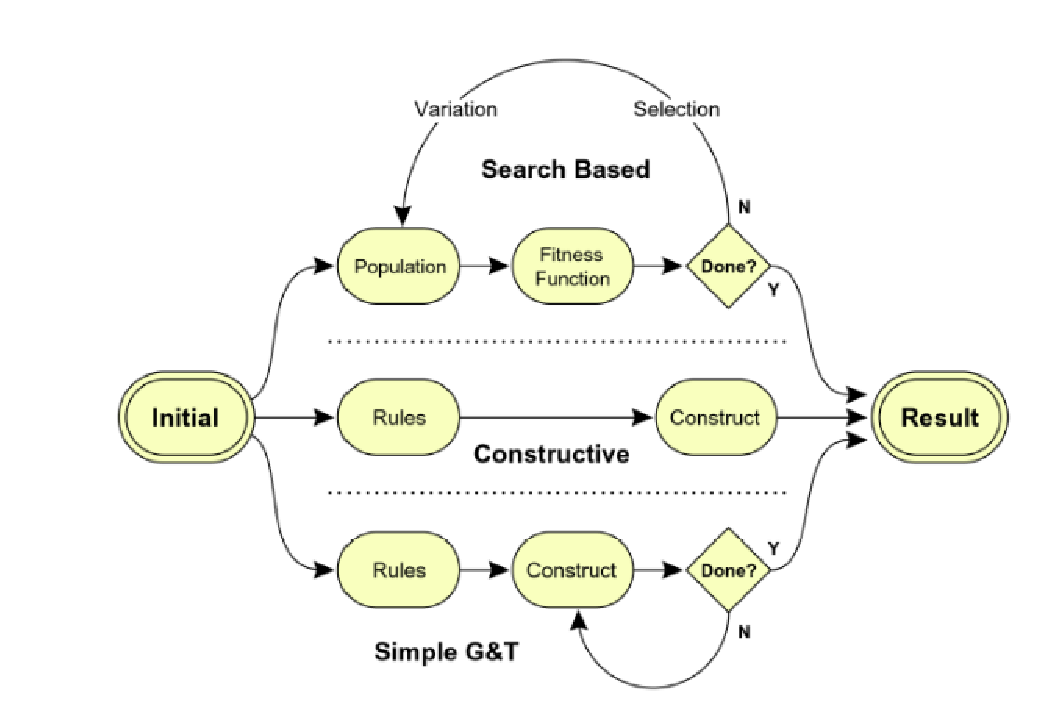
\includegraphics[width=9cm]{./eps/fig1.eps}
	\caption{Figure of ''Search-based Procedural Content Generation:
	A Taxonomy and Survey'' by
	Julian Togelius, Georgios N. Yannakakis, Kenneth O. Stanley, Cameron Browne}
	\label{Figura1}

\end{figure}

Para la generación procedural de búsquedas son necesarias unas reglas que vayan asociadas a las mecánicas de juego, por ejemplo:\\

{\bf Hom and Marks} generaron unas reglas que eran representadas en el juego y estaban basadas en una función de evaluación de simulación estática y la teoría impulsada.\\

{\bf Browne} creó un sistema de diseño de reglas para direccionamiento usando programación genética, las reglas del juego estaban representadas en árboles, el lenguaje fue formulado para el proyecto.\\

En la figura \ref{Figura2} podemos ver como se generan las reglas del juego:\\

\begin{figure}[hpb]

	\centering
	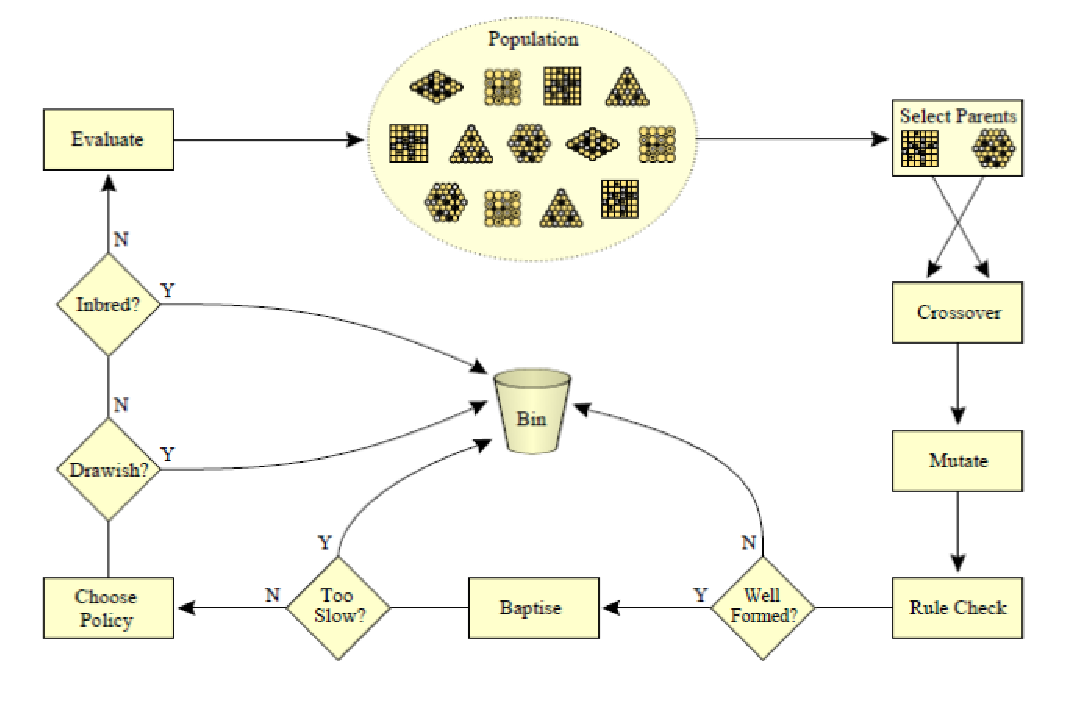
\includegraphics[width=9cm]{./eps/fig2.eps}
	\caption{Figure of ''Search-based Procedural Content Generation:
	A Taxonomy and Survey'' by
	Julian Togelius, Georgios N. Yannakakis, Kenneth O. Stanley, Cameron Browne}
	\label{Figura2}

\end{figure}

\section{Representación del espacio de búsqueda:}

Una distinción importante en la representación es entre la codificación directa o indirecta ya que una codificación directa implica una relativa simpleza computacional en el mapeo del genotipo-fenotipo, dado que en una computación compleja es necesario la creación del fenotipo desde el genotipo.\\


\section{Funciones de evaluación:}	

La evaluación es importante para ver las capacidades del algoritmo, para confirmar con garantía lo que puede crear y para comparar el contenido generado con otros contenidos.\\


Para diseñar la función de evaluación el diseñador debe primero decidir cuánto quiere optimizar para fortalecer el diseño.\\


Tres tipos de evaluación son:\\

Evaluación directa por funciones: en la que directamente una función saca el valor del fitness del contenido generado.\\

Evaluación simulada por funciones: en el que el contenido se va manipulando y se va evaluando.\\


Evaluación interactiva: mientras el juego está en ejecución se evalúa la interacción con el personaje y se van generando los contenidos.\\

\section{Construcción de terrenos y mapas:}

Una forma de representar el terreno es en forma de expresiones de árboles y la evaluación en cada punto se determina mediante la consulta de árboles de expresión evolucionando y sustituyendo las coordenadas de la posición actual por coordenadas de las constantes del árbol.\\


La  función de evaluación está basada en la {\bf teoría de accesibilidad} en la cual se evalúa el terreno en función de la pendiente.\\

Para elegir las métricas apropiadas para la medición de la construcción es necesario esforzarse en la elección de medidas lo más lejanas posibles de los parámetros de entrada al sistema.\\



	\chapter[Motores de Juego]{\label{identificadorReferenciaCruzada}
Motores de Juego}


Un motor de juego, es una herramienta software diseñada para asistir a los desarrolladores en la tarea de creación de juegos y aplicaciones gráficas\cite{B9}.

\section{Arquitectura:}

Un motor de juego está compuesto por una capa de tarjeta Hardware que representa el pc o consola sobre el que se ejecutará, una capa de drivers que son componentes Software que proporciona el sistema operativo o el proveedor de HArdware.

Por otra parte tiene el sistema operativo sobre el que está ejecutándose el juego todo el tiempo, la parte de SDKs que da soporte a la parte de programación del juego y la parte de estructuras de datos y algoritmos para dar soporte a la programación también.

Si nos centramos en la parte estética del juego, nos encontramos con una parte gráfica, una parte de animación de personajes y modelos y una parte de colisiones y física en la que se deforman los escenarios y da realismo al juego.

Sin embargo, si nos fijamos en la parte de la inteligencia artifical, nos encontramos una parte dedicada especialmente a eso, que está producida por el SDK.

Por último nos encontramos una serie de capas que ayudan a la depuración, renderizado, efectos visuales y gameplay para realizar pruebas.

En la \ref{Figura3} podemos ver como se organizan las distintas partes.

\begin{figure}[h!]

	\centering
	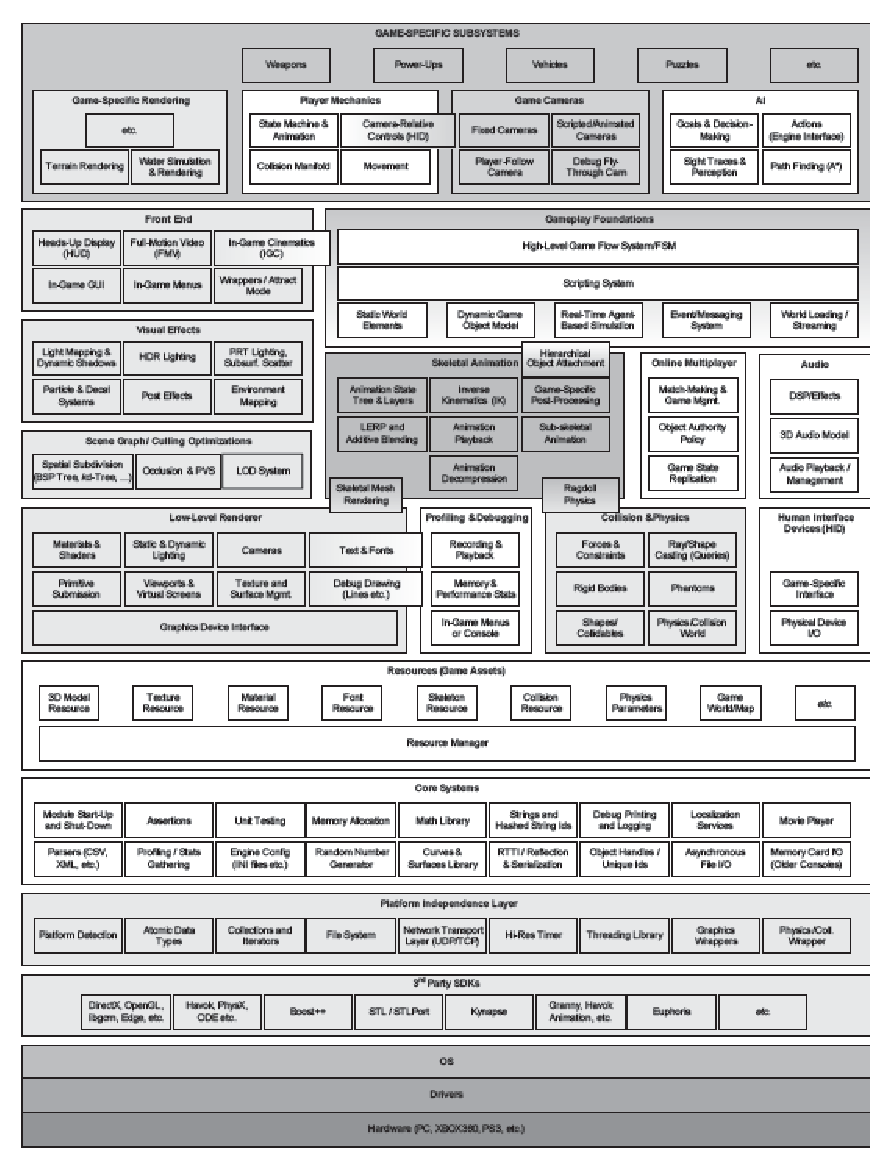
\includegraphics[width=8cm]{./eps/fig3.eps}
	\caption{Arquitectura de un motor de juegos, extraído de \cite{B10}}
	\label{Figura3}

\end{figure}
\newpage

\section{Selección de motor:}
Hay cientos de motores gráficos en el mercado y a la hora de elegir uno para el desarrollo de un proyecto hay que tener en cuenta los siguientes criterios\cite{B9}:

\begin{itemize}

	\item Si la herramienta tiene soporte o no para 2D y 3D.
	\item Si la herramienta es multiplataforma.
	\item Los lenguajes de programación que soporta la herramienta.
	\item Si tiene un motor de físicas y herramientas de inteligencia artificial.
	\item Si incorpora herramientas más avanzadas como editores de terrenos.
	\item El tipo de licencia que utiliza. 

\end{itemize}

En la tabla \ref{Tabla3} están los tres motores de juegos más importantes del mercado.

\begin{sidewaystable}[hbp]
\resizebox{20cm}{!}{ 
\begin{tabular}{| p{2cm} | p{1.5cm} | p{1.5cm} | p{2.5cm} | p{2cm} | p{2cm} | p{2cm} | p{4cm} | p{3.5cm}|}
	\hline 
		Nombre & 2D/3D & IDE & Lenguaje & Plataforma & Motor Físico & Herramientas de IA & Características Avanzadas & Licencia\\
   		\hline 
   		Unity3D & 2D y 3D & Mac y Windows & C\#, Boo, JS & Mac, Windows,
   		Linux, iOS, Android, PS3, XB360, PSP, Wii, PSVita, Flash,
   		Web & PhysX &  NavMesh y Path Finding & Forward y Deferred
   		rendering, Occlusion Culling, light mapping, light probing, LOD discreto, edición de terrenos, sistema de partículas & Comercial. Versión básica
   		gratuita (desktop y web) y versiones PRO y plataformas
   		móviles y consolas con un pago único sin royalties\\
   	\hline
    	UDK/Unreal Engine 4& 2D y 3D & Sí & Unreal Script & Mac, Windows,
    	iOS, Android, PS3, XB360, PSVita, Wii, Flash & PhysX &Path Finding &  Deferred rendering, occlusion culling, parallax mapping, Per Object Motion
    	Blur  &  Comercial. Versión libre y pago de royalties sobre producto vendido al superar un umbral de facturación. La versión Unreal Engine 3 dispone de más funcionalidades y una licencia comercial más cara.\\
    \hline
        Corona SDK & 2D & No & LUA & iOS, Android, Nook, Kindle Fire & Box2D & No. Deben ser programadas desde cero en LUA  & Interfaz simple de Lua para
        la programación de física & Comercial. Versión Indie para desarrollar para una única plataforma (iOS o Android) y versión Pro para todas las
        plataformas.\\
    \hline
\end{tabular}
}


\caption{Lista de Motores obtenida en el artículo: \cite{B9}} \label{Tabla3}
\end{sidewaystable}

Una vez que sabemos los criterios y los motores más usados del mercado, podemos disponernos a elegir un motor para nuestro proyecto.

Como el proyecto, tiene una parte en 2D, que es la de generación de planetas, necesitamos un motor que disponga de 2D, los cuales son los tres, sin embargo la parte de generación de ciudades, se hará en 3D, por lo que será necesario que disponga de 3D también,por lo que descartaremos el Corona SDK.

Por otra parte, necesitamos algo que se haga en PC, así que nos sirven los dos motores que nos quedan, pero si nos fijamos en los lenguajes de programación, Unity tiene una mayor variedad respecto a UDK que sólo soporta ''Unreal script''.

Si nos fijamos en la parte de motor de físicas, que es un motor que simula los movimientos físicos \cite{B11}, vemos que es una parte irrelevante, ya que no vamos a mover nada, ni vamos a generar movimientos sismicos, ni de personajes.

Por otra parte si nos fijamos en la parte de la inteligencia artificial, vemos que Unity tiene una mayor variedad que UDK, lo que para el proyecto nos beneficia bastante para la programación de los algoritmos genéticos, lo mismo que pasa con las características avanzadas.

Si nos fijamos en el punto de licencias, Unity cuenta con una versión gratuita para la plataforma de PC, lo que nos viene perfecto, sin embargo, UDK para ofrecernos lo mismo que Unity requiere de una subcripción.

Una vez estudiado todas las características que nos proporcionan los motores que más se usan en el mercado, podemos decir que Unity es el que más nos beneficiará para el desarrollo del proyecto.


\newpage





	%\chapter[Análisis de los algoritmos]{\label{identificadorReferenciaCruzada}
Análisis de los algoritmos}

En este capítulo nos centraremos en el análisis de los tres algoritmos explicados en el anterior, para ello haremos un anáisis a posteriori en un ordenador con las características mostradas en la tabla \ref{Tabla4}:

\begin{table}[h!]
\begin{center}
	\resizebox{5cm}{!}{ 
	\begin{tabular}{| l | r |}
		\hline 
			Procesador & Intel Core i7-2600 3.4GHz \\
				\hline 
			Memoria RAM & 32Gb DDR3 \\
		\hline
			Disco Duro &  Samsung SSD 850 EVO 120Gb\\
		\hline
			Sistema operativo.& Windows 7 profesional 64-bits\\
		\hline
			Tarjeta gráfica & Nvidia GeForce GT-430\\
		\hline
			
	\end{tabular}
	}
\end{center}
\caption{Características del ordenador} \label{Tabla4}
\end{table}

\section{Tiempos de ejecución:}

Para los algoritmos hemos realizado distintas ejecuciones con valores de la forma:

\begin{itemize}
	\item 10x10
	\item 20x20
	\item 30x30
	\item 40x40
	\item 50x50
	\item 60x60
	\item 70x70
	\item 80x80
	\item 90x90
	\item 100x100
\end{itemize}

Si nos damos cuenta, estamos realizando divisiones cada vez mayores para comprobar como aumenta el tiempo en cada algoritmo. Tras las distintas ejecuciones nos sale lo mostrado en \ref{Tabla5}

\begin{table}[h!]
\begin{center}
	\resizebox{15cm}{!}{ 
	\begin{tabular}{| c | c | c | c | c | c | c | c | c | c | c |}
		\hline 
			Algoritmo & 10x10 & 20x20 & 30x30 & 40x40 & 50x50 & 60x60 & 70x70 & 80x80 & 90x90 & 100x100 \\
				\hline 
			Primer algoritmo &  2.05	& 3.32	& 4.34	& 4.65	& 5.06	& 7.50	& 11.65	& 16.49	& 27.31	& 44.67\\
		\hline
			Segundo algoritmo & 9.47	& 24.70	& 67.09	& 155.33	& 278.37	& 446,81	& 1144.14	& 1240.22	& 1500.64	& 1924.82\\
		\hline
			Tercer algoritmo & 1.09	& 1.23	& 1.34	& 5.01	& 10.14	& 13.9	& 28.21	& 30.64	& 36.88	& 64.91\\
		\hline
	\end{tabular}
	}
\end{center}
\caption{Tiempo de ejecución (s) de los algoritmos para los distintas divisiones.} \label{Tabla5}
\end{table}


Como podemos ver, el tiempo en el segundo algoritmo es mayor, también se ha explicado anteriormente que es el más complejo, por otra parte, si representamos esos datos en gráficas de R nos daría lo mostrado en la figura \ref{Figura10}.

\begin{figure}[h!]

	\centering
	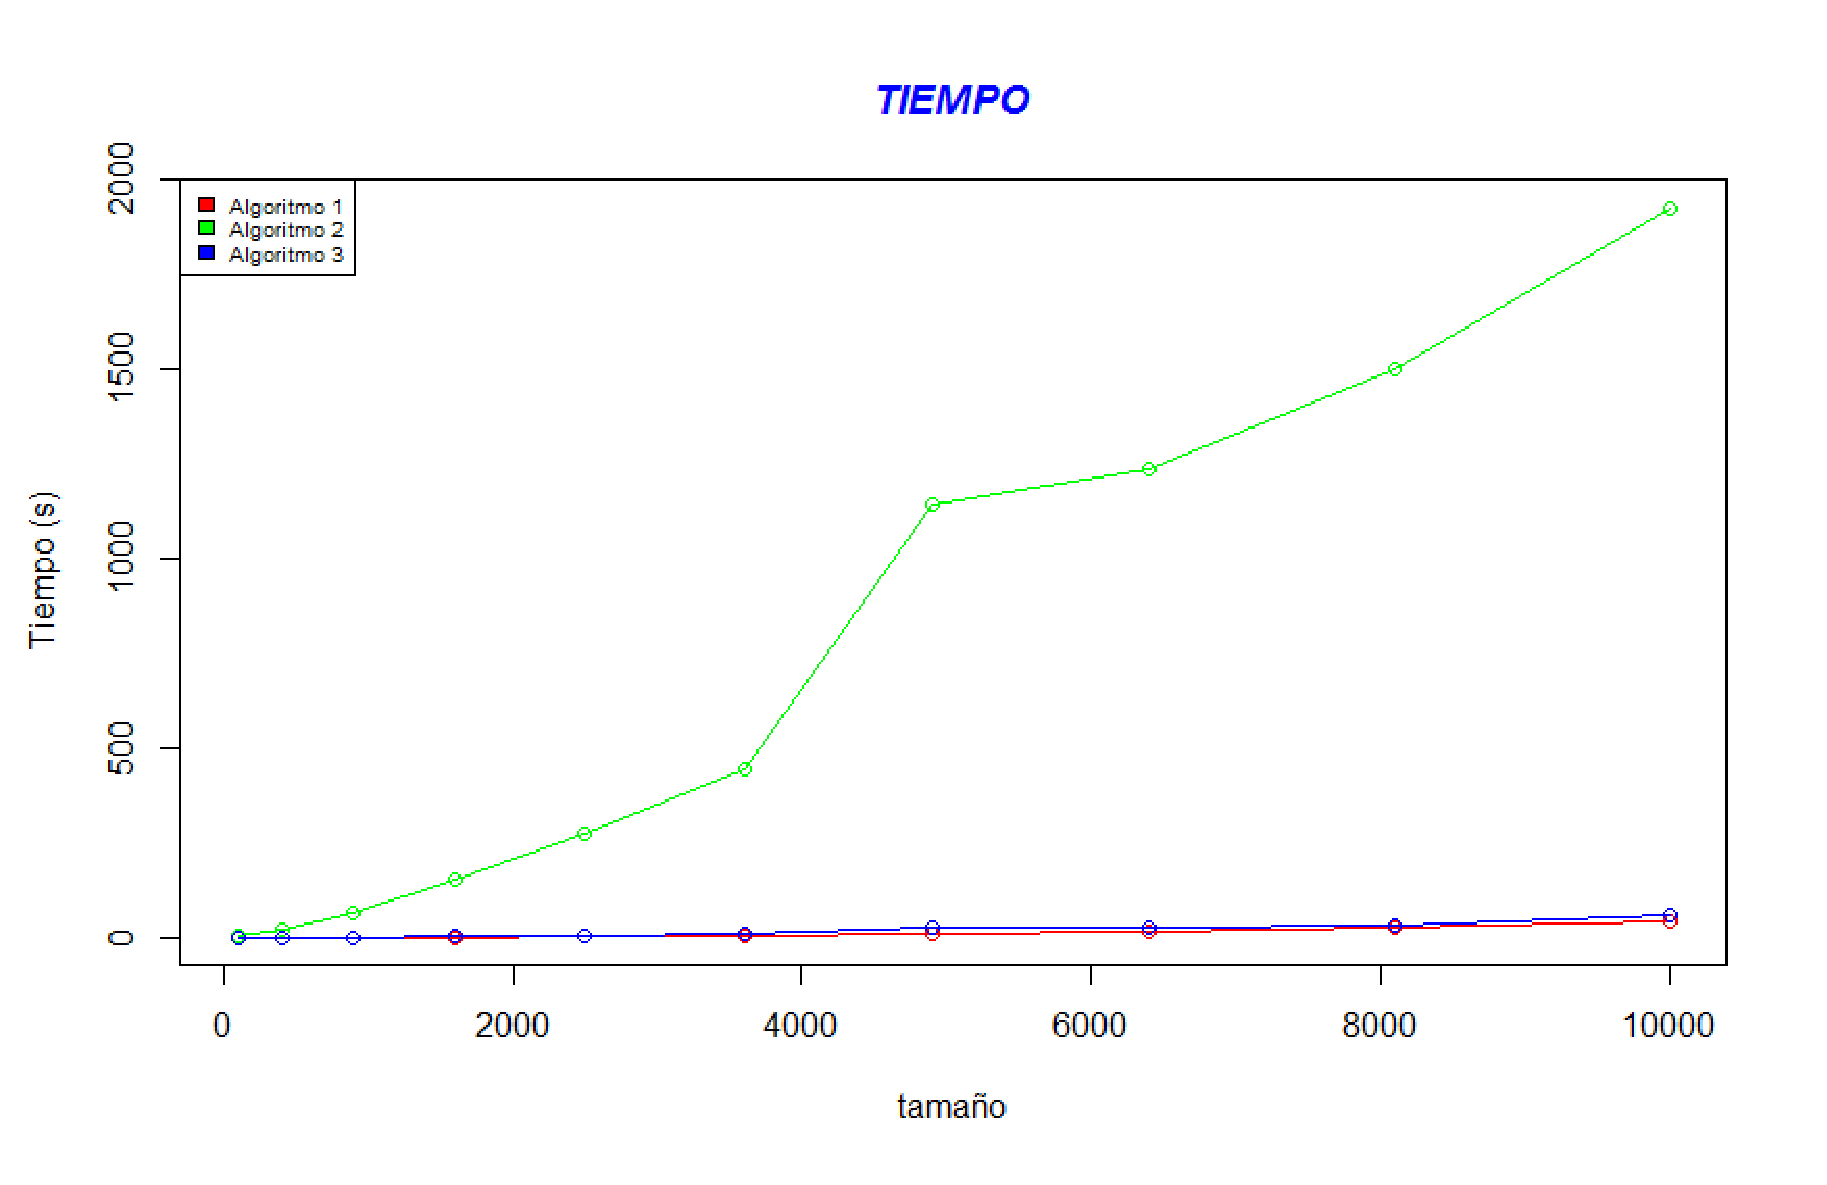
\includegraphics[width=8cm]{./eps/tiempo.eps}
	\caption{Representación gráfica en R de los tiempos de ejecución.}
	\label{Figura10}

\end{figure}

Con los datos representados, es trivial ver que los algoritmos, son de la forma \textbf{O$(n)$}. Para mostrarlo mejor, en la figura \ref{Figura11} podemos ver las gráficas de los algoritmos además del gráfico de O$(n)$ y de O$(n^2)$.

\begin{figure}[h!]

	\centering
	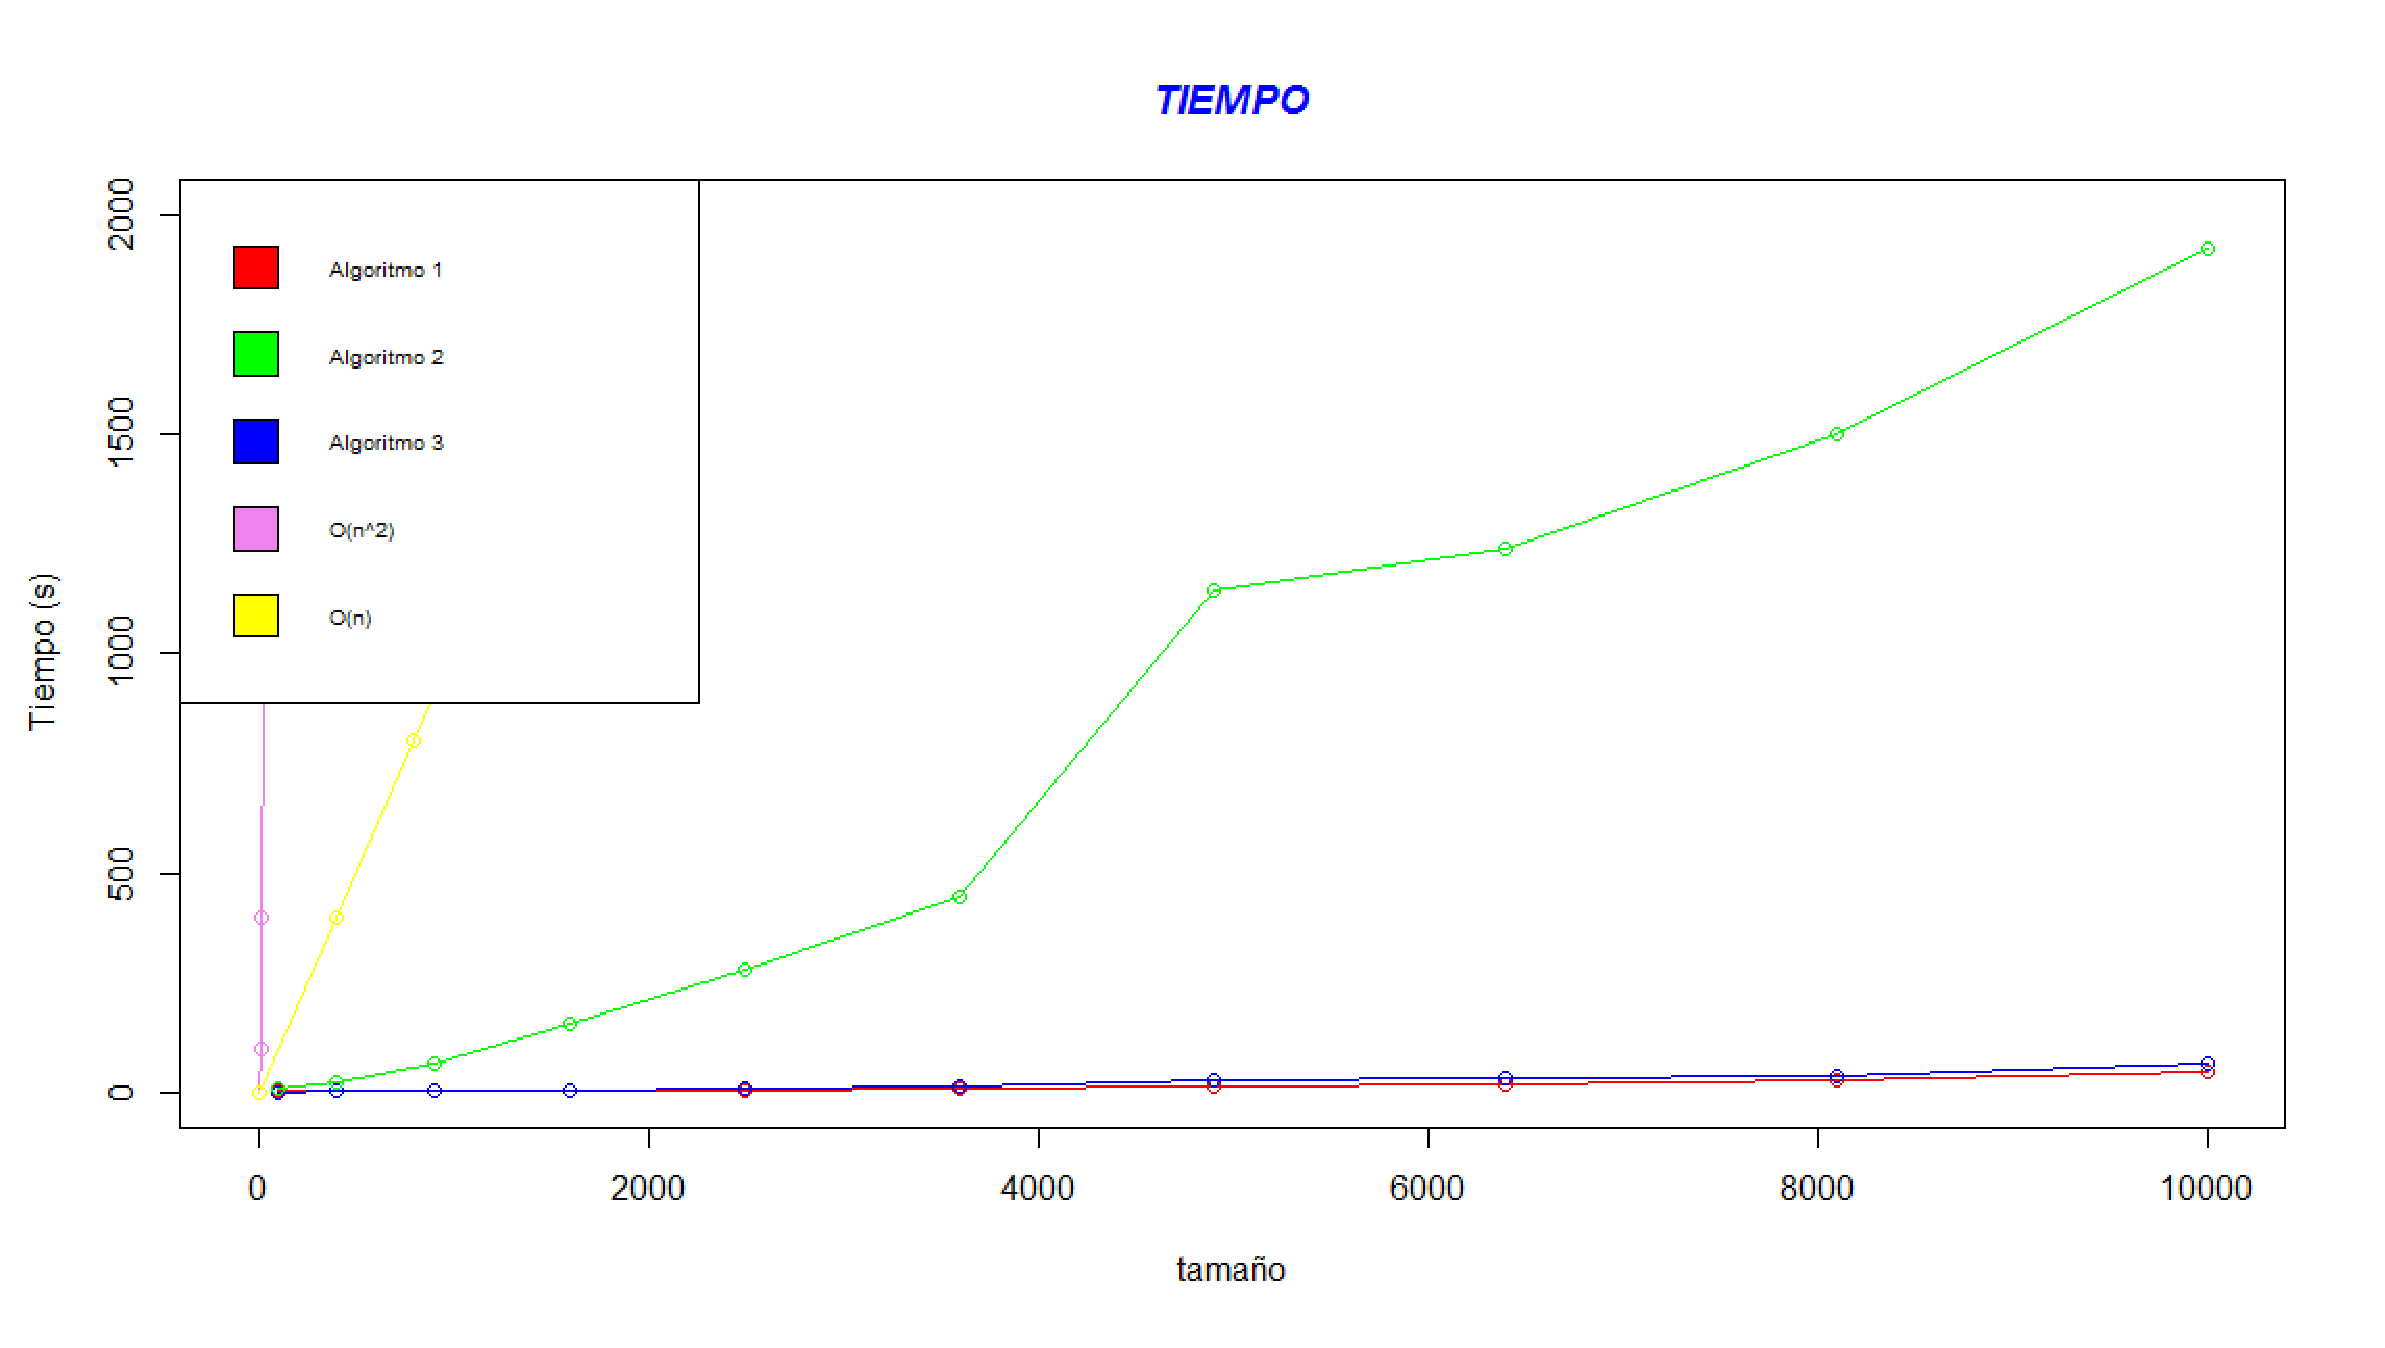
\includegraphics[width=8cm]{./eps/tiempofinal.eps}
	\caption{Comparación de tiempos con O$(n)$ y O$(n^2)$,realizada en R.}
	\label{Figura11}

\end{figure}

\section{Memoria:}

Para el estudio de la memoria utilizada por cada algoritmo hemos realizado la misma cantidad de ejecuciones con el mismo tamaño, dando los resultados indicados en \ref{Tabla6}


\begin{table}[h!]
\begin{center}
	\resizebox{15cm}{!}{ 
	\begin{tabular}{| c | c | c | c | c | c | c | c | c | c | c |}
		\hline 
			Algoritmo & 10x10 & 20x20 & 30x30 & 40x40 & 50x50 & 60x60 & 70x70 & 80x80 & 90x90 & 100x100 \\
				\hline 
			Primer algoritmo &  1.81 & 	1.85 &	1.87	& 1.95	& 2.11	& 2.23	& 2.38	& 2.53	& 2.64	& 2.82\\
		\hline
			Segundo algoritmo & 2.27 &	3.81 &	5.12	& 7.77 &	10.9 &	14.1 &	19.4 &	24.1 &	29.6	& 31.8\\
		\hline
			Tercer algoritmo & 0.5	& 0.68	& 0.80	& 1.01	& 1.25	& 1.50	& 1.93	& 2.12	& 2.28	& 2.50\\
		\hline
	\end{tabular}
	}
\end{center}
\caption{Memoria RAM (Gb) utilizada en cada ejecución de los distintos algoritmos.} \label{Tabla6}
\end{table}


Por otro lado hemos analizado la memoria que utiliza cada uno de los algoritmos en las distintas ejecuciones para que el usuario que vaya a trabajar con la biblioteca, pueda elegir que algoritmo le conviene más. En la figura \ref{Figura12} podemos ver la cantidad de memoria RAM utilizada por cada algoritmo.

\begin{figure}[h!]

	\centering
	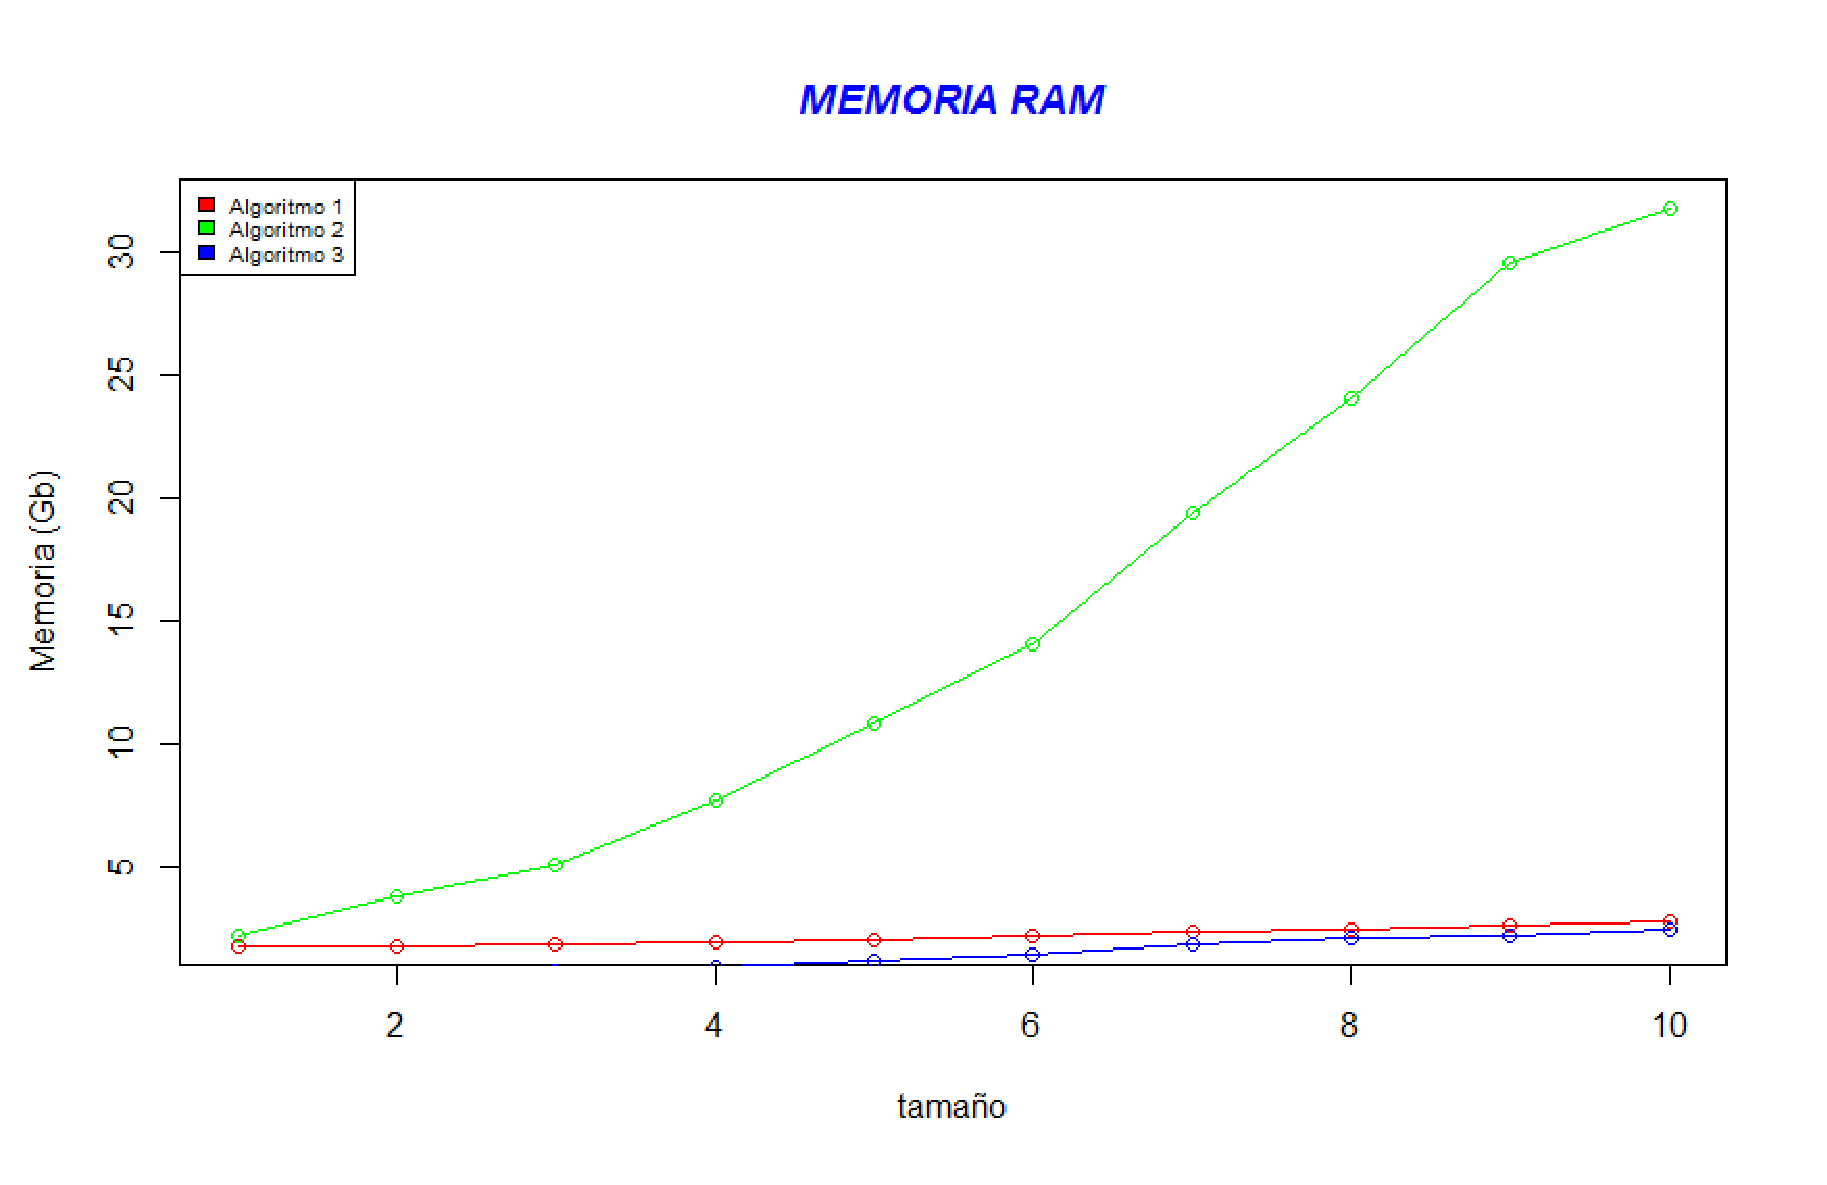
\includegraphics[width=8cm]{./eps/memoria.eps}
	\caption{Memoria RAM (Gb) utilizada por los distintos algoritmos según ejecución, realizada en R.}
	\label{Figura12}

\end{figure}

Como podemos ver, la cantidad de memoria utilizada por el segundo algoritmo, es mucho mayor, deja al ordenador casi sin memoria en la última ejecución, mientras que el primero y el tercero usan una cantidad de memoria bastante razonable y que se puede usar en cualquier juego.


\section{Conclusiones:}

Las conclusiones obtenidas de los últimos puntos son:

Los algoritmos primero y tercero pueden ser utilizados en cualquier juego, realizando tamaños de ciudades tan grandes como se deseen, mientras que el segundo algoritmo, sólo se puede utilizar en tamaños pequeños, si deseamos usarlo en cualquier juego, en el caso de querer ciudades grandes y con tanto detalle como este algoritmo nos las muestra, el juego tendría que tener calidad, y los requisitos mínimos para el funcionamiento de este serían bastante mayores.

\newpage







	%\chapter[Conclusiones y trabajo futuro]{\label{identificadorReferenciaCruzada}
Conclusiones y trabajo futuro}


Los objetivos de este trabajo eran, la contrucción de una biblioteca para generación procedural de ciudades que fuese posible usar por cualquier persona, e importar las ciudades al motor de juegos Unity 3D para que sea posible usarlo en cualquier juego que se cree con este motor. Tras la realización de este trabajo, hemos llegado a la conclusión de que los algoritmos realizados son bastante competitivos con los que hay en el mercado, aunque el segundo algoritmo en ciudades muy grandes no se podría usar en cualquier juego, dado su coste. 

El trabajo futuro que se puede añadir a este proyecto sería por una parte la construcción definitiva de algoritmos genéticos ya que los algoritmos actuales son de una única iteracción, y comprobar con costes cual de las ciudades que van saliendo con la mezcla de genes ''edificios'', para obtener ciudades aún más competitivas, por otra parte este algoritmo se usará para la generación de varios juegos que se encuentran actualmente en desarrollo y que esperemos que el año que viene uno de ellos se encuentre en la plataforma de videojuegos ''STEAM'', para su venta y distribución. Todo el trabajo realizado se encuentra en GitHub en \cite{B13}.
	%\include{pfg_main_060}


	% INCLUIMOS LOS APÉNDICES...
        \appendix
	%%
% Memoria económica.
%

\chapter[Título de apéndice]{
	Título de apéndice.
}

Lorem ipsum dolor sit amet, consectetur adipiscing elit. Integer luctus varius augue vel imperdiet. Maecenas neque turpis, accumsan ut eleifend vel, eleifend gravida est. Duis mattis pulvinar porta. Nunc consequat, felis ut malesuada egestas, ipsum urna sodales enim, eu lobortis mauris tellus in augue. In tristique tortor id nisi placerat et rutrum tortor auctor. Aenean erat elit, faucibus non egestas semper, volutpat sit amet ante. Nam nulla justo, suscipit nec sagittis sed, varius id magna. Duis a lorem id felis eleifend aliquet eget vel arcu. Etiam ultricies diam a magna facilisis ornare. Integer tempor massa quis sem gravida bibendum. Sed massa felis, condimentum sit amet bibendum in, tristique sit amet mauris. Nullam tellus ante, ornare eget mollis ac, gravida id nunc. Donec elit neque, aliquam eget auctor sed, gravida in nibh. Vestibulum sit amet diam a magna tempor bibendum quis a ante. Integer augue sapien, facilisis ac malesuada sed, consectetur id turpis. Quisque a leo dapibus felis aliquet vestibulum vitae vitae urna. Nunc ut felis ut metus gravida ultricies. Cras tincidunt nisi ante. Nunc eu quam interdum dui cursus lacinia. Praesent adipiscing ultrices nulla at posuere.

Aliquam gravida facilisis eleifend. Nunc id lorem nibh. Nulla facilisi. Nunc suscipit lectus quis tellus adipiscing adipiscing. Proin ipsum justo, egestas dictum iaculis et, pretium non diam. Aenean vehicula hendrerit lectus, vel bibendum nisi volutpat quis. Fusce molestie condimentum libero, nec scelerisque nisi mollis et. Aliquam placerat accumsan congue. In scelerisque nulla sit amet mauris consectetur consectetur. Suspendisse mattis mi in sapien egestas sit amet accumsan urna sagittis. Mauris metus massa, porta at rutrum eget, sollicitudin eu risus. Donec non diam erat. Nam sagittis, nibh non fermentum ornare, ipsum est mollis felis, eget vulputate tellus ante at erat. Praesent porta tempus velit at faucibus. Donec rhoncus varius nunc, eget imperdiet ligula blandit eget. Morbi pulvinar, nunc ac porta interdum, mauris ligula sollicitudin sem, et sollicitudin turpis magna eu lectus. Pellentesque nulla dui, feugiat quis pharetra eu, accumsan imperdiet quam. Aenean lacinia porttitor leo vitae hendrerit. Pellentesque dictum ultricies dui, et rhoncus nulla sagittis ut. Suspendisse suscipit, risus sed posuere rhoncus, neque metus scelerisque diam, eu gravida quam orci eu dui.

Nulla sit amet sem massa, aliquet auctor magna. Vivamus quis magna sollicitudin felis bibendum mollis. Etiam elementum lacus id quam tincidunt pulvinar. Ut vehicula aliquam ante, vel venenatis libero bibendum eget. Sed gravida lobortis velit, et ornare nunc ullamcorper et. Morbi neque sapien, mattis id semper in, varius at arcu. Duis aliquam ornare sem, eu sagittis libero facilisis non. Nunc quis ultricies augue. Pellentesque ac nulla libero, ut suscipit dui. Morbi aliquet quam non metus iaculis quis accumsan ipsum consectetur.

Mauris mauris odio, varius quis accumsan bibendum, vulputate vel tellus. Sed non consectetur eros. Aenean et mi ut est tincidunt commodo. Donec nunc metus, facilisis a consequat vitae, dignissim quis leo. Cras condimentum, felis a molestie viverra, massa eros consequat nisl, at porta nibh sapien condimentum ante. Duis convallis velit quis metus pulvinar convallis. Suspendisse sed purus non purus dictum ultricies in vitae nisl. Cras convallis erat eu ipsum molestie fermentum. Mauris turpis nunc, condimentum non aliquam ac, ornare at lectus. Donec scelerisque fermentum malesuada. Praesent urna nisl, iaculis sed pharetra eu, tincidunt et lectus. Nulla posuere eros at elit vehicula laoreet. Sed ut erat orci, ac pellentesque nibh. Nulla at sapien sed justo luctus laoreet.

Sed convallis massa laoreet mi venenatis eget dapibus orci varius. Pellentesque purus nisi, placerat nec pretium ac, pretium vitae augue. Vivamus eleifend vestibulum mi, ac dignissim urna vulputate vel. Integer volutpat neque purus. Nulla hendrerit tempus est nec aliquet. Ut facilisis bibendum nisl eget porttitor. Cum sociis natoque penatibus et magnis dis parturient montes, nascetur ridiculus mus. Fusce consectetur sem eget ante rhoncus nec mollis lorem volutpat. Fusce in libero lectus, ut gravida lectus. Nam nulla nunc, dignissim sed sollicitudin a, commodo vel felis. Donec lacinia justo quis neque tempor interdum ut cursus mi. Phasellus venenatis porttitor mi consectetur egestas. Pellentesque quis elit nibh. Pellentesque molestie turpis ac arcu gravida sed ultricies felis pulvinar.

%         \include{pfg_appendix_020}


	% INCLUIMOS LA BIBLIOGRAFÍA...
	\nocite{*}	% Se usa para indicar en la bibliografía las referencias no citadas.
	\bibliography{pfg_biblio}
	\bibliographystyle{plain}
	

\end{document}

